% ****** Start of file apssamp.tex ******
%
%   This file is part of the APS files in the REVTeX 4.2 distribution.
%   Version 4.2a of REVTeX, December 2014
%
%   Copyright (c) 2014 The American Physical Society.
%
%   See the REVTeX 4 README file for restrictions and more information.
%
% TeX'ing this file requires that you have AMS-LaTeX 2.0 installed
% as well as the rest of the prerequisites for REVTeX 4.2
%
% See the REVTeX 4 README file
% It also requires running BibTeX. The commands are as follows:
%
%  1)  latex apssamp.tex
%  2)  bibtex apssamp
%  3)  latex apssamp.tex
%  4)  latex apssamp.tex
%
\documentclass[%
 reprint,
%superscriptaddress,
%groupedaddress,
%unsortedaddress,
%runinaddress,
%frontmatterverbose, 
%preprint,
%preprintnumbers,
%nofootinbib,
%nobibnotes,
%bibnotes,
 amsmath,amssymb,
 aps,
 pra,
%prb,
%rmp,
%prstab,
%prstper,
%floatfix,
]{revtex4-2}
\usepackage[spanish,es-nodecimaldot]{babel}
\usepackage{color,soul}
\usepackage{physics}
\usepackage{minted}
\usepackage{graphicx}% Include figure files
%\usepackage{svg}
\usepackage{dcolumn}% Align table columns on decimal point
\usepackage{bm}% bold math
\usepackage{hyperref}% add hypertext capabilities
\definecolor{linkcolour}{rgb}{0,0.2,0.6} % Link color
\hypersetup{colorlinks,citecolor=linkcolour,breaklinks,urlcolor=linkcolour,linkcolor=linkcolour}
\usepackage{color,soul}
\usepackage{soulutf8}
%\usepackage[mathlines]{lineno}% Enable numbering of text and display math
%\linenumbers\relax % Commence numbering lines

%\usepackage[showframe,%Uncomment any one of the following lines to test 
%%scale=0.7, marginratio={1:1, 2:3}, ignoreall,% default settings
%%text={7in,10in},centering,
%%margin=1.5in,
%%total={6.5in,8.75in}, top=1.2in, left=0.9in, includefoot,
%%height=10in,a5paper,hmargin={3cm,0.8in},
%]{geometry}

\begin{document}

\preprint{APS/123-QED}

\title{Oscilador armónico cuántico unidimensional en baño\\térmico usando el algoritmo Metrópolis.}% Force line breaks with \\

\author{Juan Esteban Aristizabal Zuluaga}
\affiliation{Instituto de Física, Universidad de Antioquia.}%Lines break automatically or can be forced with \\

\date{\today}% It is always \today, today,
             %  but any date may be explicitly specified

\begin{abstract}
En este artículo presentamos un estudio del oscilador armónico cuántico unidimensional en un baño térmico. En particular, nos interesamos por calcular la probabilidad de encontrar el sistema en una posición dada. Para esto, presentamos los cálculos teóricos cuánticos y su contraparte clásica, con el fin de comparar los resultados. Especialmente nos enfocamos en usar el algoritmo Metrópolis para reconstruir histogramas que representan las distribuciones de probabilidad cuánticas, tanto en el espacio de posiciones como en los niveles de energía. Estos resultados cuánticos los usamos para contrastarlos con los clásicos y los tres casos presentados   –baja, media y alta temperatura– concuerdan claramente con los cálculos teóricos. Se presenta también la implementación del algoritmo Metrópolis en el lenguaje de programación «Python». 
\begin{description}
\item[Palabras clave] 	Oscilador armónico, física estadística cuántica, baño térmico, ensamble \\
						canónico, algoritmo Montecarlo.
\end{description}
\end{abstract}

%\keywords{Suggested keywords}%Use showkeys class option if keyword
                              %display desired
\maketitle

%\tableofcontents

\section{\label{sec:Intro}Introducción}
El oscilador armónico ha sido históricamente para la física un sistema simple pero del que se puede extraer gran cantidad de información y con el que se han descubierto muchos nuevos métodos y hasta teorías completas, basadas en los razonamientos y el conocimiento obtenido de éste. Por citar un ejemplo, está la cuantización del campo electromagnético que se puede reducir a un sistema «osciladores armónicos» no acoplados y en general las teorías de segunda cuantización en la base número usan gran parte del formalismo del oscilador armónico cuántico, aunque con un significado muy diferente al que se le da en el sistema que nos compete\cite{Grynberg2010,Schwartz2013}. 

En nuestro caso hemos tomado el oscilador armónico unidimensional inmerso en un baño térmico y hemos estudiado su comportamiento a diferentes temperaturas y contrastado los resultados cuántico y clásico para la probabilidad de encontrarlo en una posición dada. Para ello hemos revisado los resultados teóricos. Entre diferentes alternativas presentadas en la literatura para llegar al resultado cuántico, entre ellas el formalizmo de intrgrales de camino \cite{Barone2003,Holstein1998}, propagadores \cite{Kheirandish2018}  y métodos más heurísticos como el de Feynman \cite{RichardP.Feynmann1972}, hemos decidido presentar el formalismo desarrollado por Cohen-Tannoudji \cite{Cohen-Tannoudji}, el cual deriva una ecuación diferencial parcial para encontrar los elementos de matriz diagonales del operador densidad, los cuales corresponden con la probabilidad en la que estamos interesados. El método que presentamos tiene la ventaja de que requiere de cálculos básicos y no de métodos avanzados, que pueden ser un poco más confusos.

Por otro lado, como sabemos, en la física estadística las herramientas computacionales han permitido un mejor entendimiento de diversos problemas. En particular, el algoritmo Metrópolis ha sido ámpliamente usado desde que  Metropolis \textit{et al.} publicaron el artículo que lo propone \cite{Metropolis1953}, en el año 1953, que posteriormente gananó más popularidad con la generalización hecha en 1970 por Hastings \cite{Hastings1970}. El algoritmo es útil especialmente en problemas de alta dimensionalidad para muestrear distribuciones de probabilidad en el que otros métodos no son igual de eficientes o simplemente no funcionan –uno de los ejemplos más comunes es la implementación de este algoritmo en sistemas tipo Ising \cite{Newman1999}–, aunque en teoría se puede usar para sistemas con cualquier dimensionalidad. 

En nuestro caso, a pesar de tener un sistema de baja dimensionalidad, usamos el algoritmo metrópolis para obtener los histogramas de las densidades de probabilidad para el caso cuántico tanto para $T=0$ como varios valores de $T \neq 0$.  Por otro lado, usando el mismo algoritmo, encontramos histogramas para los niveles de energía en cada caso y comprobamos que corresponden con la distribución de Boltzmann \textit{i.e.} la distribución de probabilidad dada por el ensamble canónico de la física estadística.

La estructura del artículo es la siguiente: en la sección \ref{sec:Teoria} presentamos los resultados teóricos para la densidad de probabilidad cuántica y clásica de encontrar el oscilador armónico unidimensional en una posición dad cuando éste está inmerso en un baño térmico. En la parte \ref{sec:Resultados} contrastamos los resultados teóricos clásico y cuántico con simulaciones usando el algoritmo Montecarlo para la parte cuántica, para diferentes valores de temperatura. En esta sección también comprobamos los resultados y los límites de alta y baja temperatura que obtuvimos en \ref{sec:Teoria}. En \ref{sec:conclusion} presentamos la conclusión del trabajo y, finalmente, en los apéndices \ref{appx:codigo_matrix_squaring} y \ref{appx:codigo_temperatura_finita} escribimos las implementaciones de los algoritmos de metrópolis usados (en Python3) para generar las figuras y para los análisis de la sección \ref{sec:Resultados}.


\section{\label{sec:Teoria}Consideraciones teóricas}

Consideraremos los sistemas en unidades reducidas, es decir, con sus variables adimensionalizadas.

\subsection{Caso Clásico} \label{subsec:caso-clasico}


\subsection{Caso cuántico} \label{subsec:caso-cuantico}


\section{\label{sec:Resultados}Resultados y discusión}


\subsection{Límite de muy baja temperatura \texorpdfstring{$T \rightarrow 0$}{T tendiendo a cero}\label{subsec:limite-T-0}}

\subsection{Temperatura finita \texorpdfstring{$T \neq 0$}{T diferente de cero}\label{subsec:temperatura-finita}}


\begin{figure}[t]
	\centering
	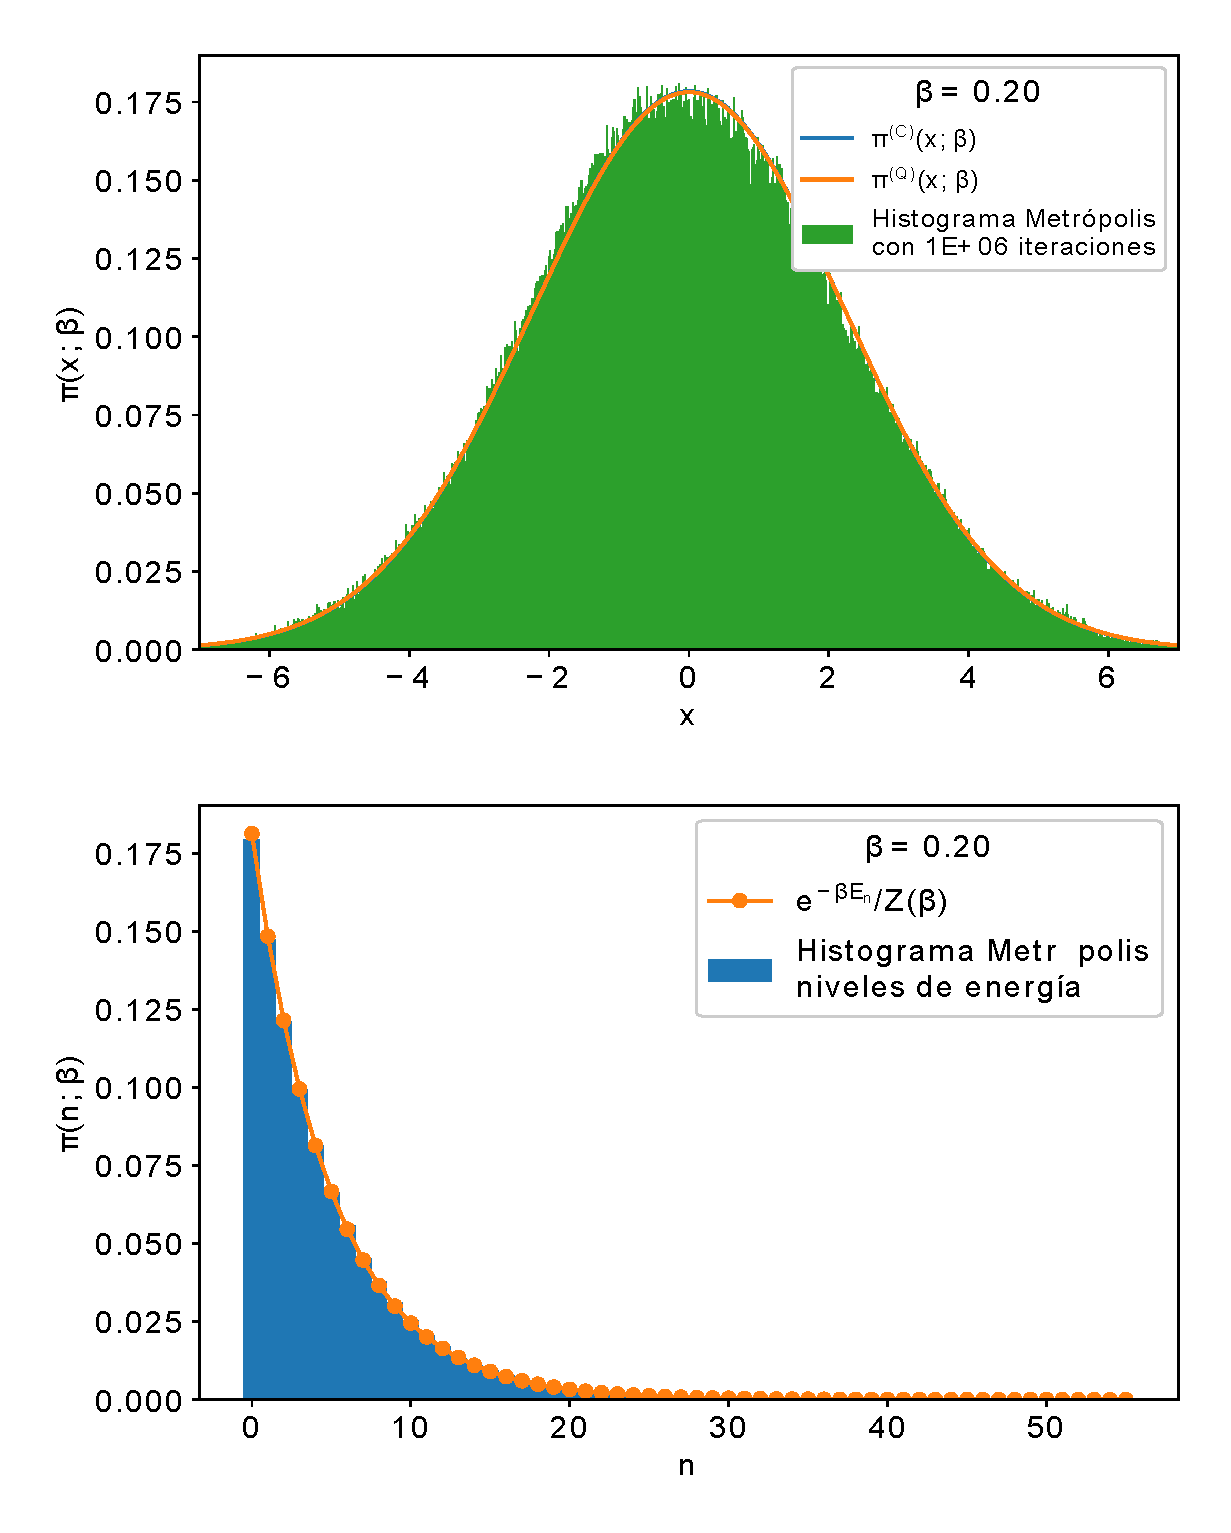
\includegraphics[width=\linewidth]{figures/0_plot_QHO_finite_temp_beta_0_20}
	\caption{Arriba: densidad de probabilidad de encontrar a la «partícula» cuántica en una posición dada, cuando está en presencia de un potencial armónico y de baño térmico a temperatura definida por $\beta=1/T=0.2$. Mostramos los resultados teóricos clásico y cuántico como línea continua y el histograma que resulta del algoritmo Metrópolis usando $10^6$ iteraciones y $\delta x = 0.5$. Observamos que éste es un límite de alta temperatura ya que las distribuciones teóricas clásica y cuántica se solapan en gran medida y son muy similares. Abajo: histograma de niveles de energía obtenido con algoritmo Metrópolis y los respectivos valores teóricos. Notamos que muchos niveles de energía contribuyen en este caso que hemos considerado de alta temperatura. Además, los valores calculados por el algoritmo se acercan en gran medida a los teóricos}
	\label{fig:beta_0.2}
\end{figure}

Como comentario final de esta sección, es importante también mencionar que los algoritmos se ejecutaron en Python3 v3.6.

\section{Conclusión\label{sec:conclusion}}

En este trabajo estudiamos el problema del oscilador armónico en un baño térmico, tanto de forma clásica como cuántica y con un tratamiento teórico y computacional –éste último en el marco del algoritmo Metrópolis.

Pudimos calcular para el oscilador armónico cuántico en un baño térmico los elementos diagonales del operador densidad en la base de posiciones, $\rho(x,x;\beta)$. Estos elementos diagonales los interpretamos como la densidad de probabilidad de encontrar a la «partícula» en la posición $x$: $\pi^{(Q)}(x;\beta)$. En el caso clásico calculamos esta probabilidad con ayuda de la función de distribución en el espacio de fase definida por el ensamble canónico. Encontramos que el límite de baja temperatura para el caso clásico es una delta de Dirac centrada en el origen, mientras que en el caso cuántico este límite corresponde con la densidad de probabilidad de la autofunción de energía del estado base del oscilador armónico, conforme se espera. De igual modo pudimos notar que en el límite de altas temperaturas la densidad de probablididad cuántica mencionada tiende a la clásica, conforme se espera también desde la física estadística. 

Para contrastar los resultados teóricos usamos el algoritmo Metrópolis para reconstruir los histogramas del sistema cuántico en el espacio de las posiciones y en los niveles de energía. Para los casos de $\beta$ evaluados encontramos que uno corresponde a un límite de alta temperatura ya que las distribuciones cuántica y clásica eran muy parecidas, también tenemos un caso intermedio entre alta y baja temperatura y uno de baja temperatura. Esas conclusiones las soportamos tanto en las comparaciones de las curvas teóricas como en los histogramas generados. Siempre los histogramas de los niveles de energía corresponden con el límite que tratamos: altas temperaturas implican contribuciones apreciables de muchos niveles de energía, mientras que para bajas temperaturas contribuyen solo niveles muy próximos al estado base.

Las implementaciones de los algoritmos usados son suficientemente generales y se podrían adaptar con cierta facilidad a otros sistemas de interés que sean objeto de estudio.

\section*{Agradecimientos}
Agradezco a mis compañeros de clase con los que tuve discusiones que ayudaron en la implementación del algoritmo y en las conclusiones presentadas. 

\nocite{*}

\bibliography{5-Semestre_X_2020_I-Fisica_Estadistica_Avanzada-Tarea_2}% Produces the bibliography via BibTeX.

\newpage



\appendix

\begin{widetext}

\section{Código 1: Matrix Squaring\label{appx:codigo_matrix_squaring}}

\inputminted[linenos,breaklines]{python}{code_1.py}

\section{Código 2: Naive Path Integral Montecarlo Sampling\label{appx:codigo_temperatura_finita}}

%\inputminted[linenos,breaklines]{python}{code_2.py}

\end{widetext}


\end{document}
%
% ****** End of file apssamp.tex ******
